\documentclass[a4paper,12pt]{report} % format a4, taille du texte, type de document
\usepackage[utf8]{inputenc} % afficher les accents correctement
\usepackage[T1]{fontenc} % police contenant caractères spéciaux français
\usepackage[francais]{babel} % langue du texte
\usepackage[colorlinks=true]{hyperref} % activer les liens hypertextes
\usepackage{graphicx} % importer les images
\usepackage{phdthesis}  %templte utilisé
\usepackage[hcentering,textwidth=150mm,textheight=225mm]{geometry} %marges
\usepackage[Bjornstrup]{fncychap} %affiche les chapitres differement
\usepackage{tocloft} %affichage different pour la table des marères
\usepackage{caption} 
\usepackage{lipsum}
\usepackage{listings}
\usepackage{color}
\usepackage{lscape}
\usepackage[scaled]{helvet}
\renewcommand\familydefault{\sfdefault} 
\setlength\parindent{0pt}

\cfoot{\thepage}

%\rhead{Rapport de stage ST50}
\lfoot{\textbf{UTBM ST50}}
\cfoot{}

\setcounter{secnumdepth}{3}

\renewcommand{\cfttoctitlefont}{\center\large\bfseries\MakeUppercase} % change toc title to upper case

\hypersetup{
  colorlinks,
  linkcolor=wine-stain,
  linktoc=all
}

\definecolor{dkgreen}{rgb}{0,0.6,0}
\definecolor{gray}{rgb}{0.5,0.5,0.5}
\definecolor{mauve}{rgb}{0.58,0,0.82}

\lstdefinestyle{custompython}{frame=tb,
  language=Python,
  aboveskip=3mm,
  belowskip=3mm,
  showstringspaces=false,
  columns=flexible,
  basicstyle={\small\ttfamily},
  numbers=none,
  numberstyle=\tiny\color{gray},
  keywordstyle=\color{blue},
  commentstyle=\color{dkgreen},
  stringstyle=\color{mauve},
  breaklines=true,
  breakatwhitespace=true,
  tabsize=3
}

\lstdefinestyle{customruby}{frame=tb,
  language=Ruby,
  aboveskip=3mm,
  belowskip=3mm,
  showstringspaces=false,
  columns=flexible,
  basicstyle={\small\ttfamily},
  numbers=none,
  numberstyle=\tiny\color{gray},
  keywordstyle=\color{blue},
  commentstyle=\color{dkgreen},
  stringstyle=\color{mauve},
  breaklines=true,
  breakatwhitespace=true,
  tabsize=3
}

\definecolor{Darkblue}{rgb}{0,0,0.4}
\definecolor{wine-stain}{rgb}{0.5,0,0}

\begin{document}

\tableofcontents

%!TEX root =/Users/ludovicl/Dropbox/Cours/UTBM/P15/RapportStage/main.tex

\newpage

\section*{Introduction}

Dans le cadre de ma formation d’ingénieur à l’Université de Technologie de Belfort Montbéliard j’ai dû effectuer un stage de vingt-six semaines à l’issue de la dernière année de mon cycle d’ingénieur. Ce stage m'a permis de me familiariser d'avantage avec le monde de l’entreprise et de mettre en pratique les connaissances acquises tout le long de mon cursus scolaire.
\\
J’ai effectué mon stage au sein de de la startup Tech4Team située à Paris.
\\ 

\indent Durant ce stage j'ai eu l'occasion de travailler avec des technologies comme Ruby on Rails, Python, PostgreSQL, Riak, différentes API,...
\\ \\
Dans la première partie de ce rapport, je présenterai l’entreprise Tech4Team en faisant un bref aperçu des logiciels développés et de l'organisation de l'équipe.
Ensuite j'aborderais les aspects plus technique avec le travail que j'ai eu à effecteur et les problèmes que j'ai rencontrés et eu a traiter.

Je terminerai pas une conclusion, les résultats et ferait le bilan de ce stage.


%\\
%Dans la deuxième partie j’évoquerai la constitution du pôle R&D de Parkeon, les interactions entre les différentes équipes ainsi que les activités et les méthodes de développement de l’équipe lecteur.
%
%
%
%Par la suite je développerai mon sujet de stage en indiquant comment j’ai acquis des compétences sur les logiciels en cours de développement par l’équipe lecteur. J’indiquerai aussi mon rôle dans les tests de la nouvelle sécurité d’échange des données.
%\\
%Pour terminer, je ferai un point sur les résultats que j’ai obtenus à l’issu de ces vingt-quatre semaines de stage et je présenterai ce que mon travail apporte à l’entreprise.

\newpage
\section*{Remerciements}
Je tiens à remercier Kevin Vitoz et Ludovic Bordes, qui m'ont fait confiance, m'ont bien accueilli et m'ont fait découvrir leur entreprise.
\\ \\ 
Je remercie également Marwan Rabbaa pour ses précieux conseils techniques, et son soutien.
%!TEX root =/Users/ludovicl/Dropbox/Cours/UTBM/P15/RapportStage/main.tex


\chapter{Présentation de l'entreprise}


Tech4Team est une startup fondée en juillet 2013 par deux entrepreneurs. Elle propose aujourd'hui deux produits majeurs Inventor-e et Arenametrix.

\section{Inventor-e}
Inventor-e est un logiciel de gestion de planning, de suivi d’états des lieux et de pilotage de maintenance. Il est conçu pour les infrastructures sportives et culturelles multifonctions.

Le logiciel fonctionne sur le principe de client-serveur. L'utilisateur utilise une tablette Android pour faire un état des lieux ou visualiser son planning. Les photos et autres données sont ensuite synchronisées dans une base de données sur un serveur distant. Il est alors possible pour l'utilisateur de visualiser les informations depuis un portail web.

\begin{center}

\includegraphics[scale=0.7]{images/inventore.png}
\captionof{figure}{Principe de fonctionnement d'inventor-e}
\label{inventore}
\end{center}

D'une manière plus technique l'application est développée pour Android 4.0 ou ultérieur, la base de données utilise PostegreSQL et l'interface web est développée avec le framework Ruby on Rails.

\section{Arenametrix}
Arenametrix est une solution logicielle, flexible, clé en main et intégrée de Big Data (analyse et exploitation des données billetteries), disponible en SaaS, pour la connaissance et la fidélisation des publics, la prospection ciblée et la mise en place d'une nouvelle politique de tarification

Arenametrix de décompose en trois briques technologiques indépendantes ou combinées : 
\begin{itemize}
  \item[\textbullet] Arena-public : Socle e-CRM
  \item[\textbullet] Arena-prospection : Prospection ciblée
  \item[\textbullet] Arena-pricing : Tarification dynamique
\end{itemize}

\begin{center}
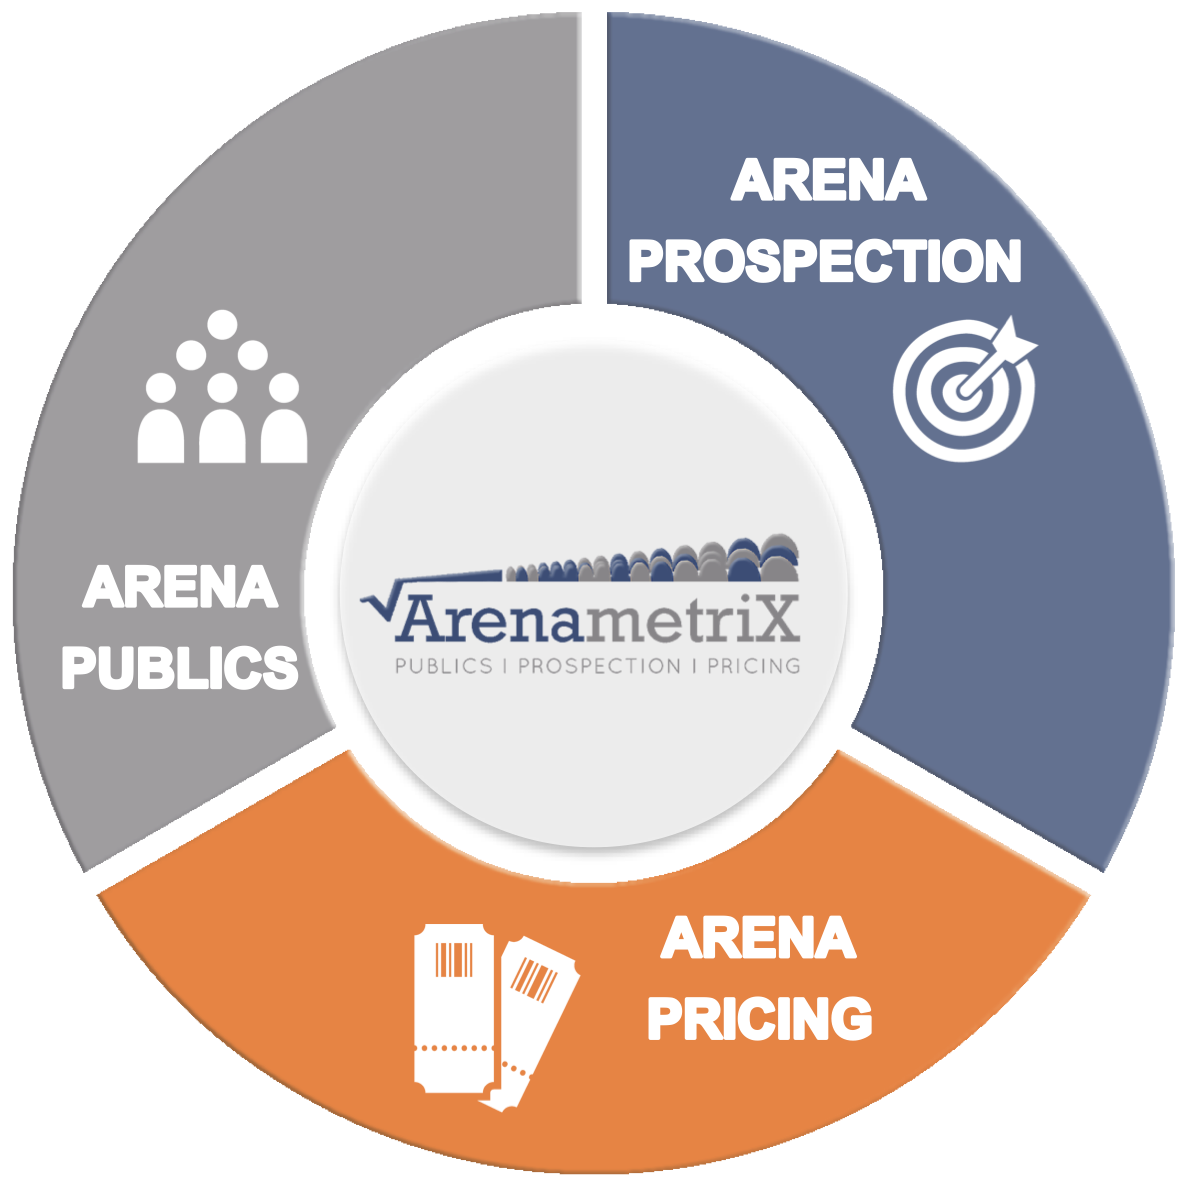
\includegraphics[scale=0.45]{images/arenametrix.png}
\captionof{figure}{Vision à 360\ensuremath{^\circ}  de Arenametrix}
\label{arenametrix}
\end{center}

\subsection{Arena-public}
Arena-public est le socle e-CRM d’exploitation des données publics.

Il permet :
\begin{itemize}
  \item[\textbullet] La centralisation des données publics, B to B et B to C
  \item[\textbullet] Le nettoyage et enrichissement des données (sexe, âge, lieu de résidence, fréquentation du stade, dépenses merchandising…)
  \item[\textbullet] La visualisation graphique de la base de données à 360\ensuremath{^\circ}
  \item[\textbullet] L'analyse mono-variable et bi-variable en croisant des données identitaires et de consommation
\end{itemize}

\subsection{Arena-prospection}
Module d’optimisation du démarchage commercial.

Ce module permet :
\begin{itemize}
  \item[\textbullet] La sélection d’une liste de contacts
  \item[\textbullet] Le classement des prospects selon leur probabilité de souscription
  \item[\textbullet] La gestion interfacée d’une campagne de téléprospection, de mailing et de SMS auprès des prospects
  \item[\textbullet] L'analyse des retours : réaction au démarchage, taux de conversion et intégration à la priorisation
\end{itemize}

\subsection{Arena-pricing}
Module de yield management.

Ce module permet :
\begin{itemize}
  \item[\textbullet] La création de typologies de publics par segmentation et profilage
  \item[\textbullet] La prévision de la demande en billets pour un événement
  \item[\textbullet] Recommandations tarifaires en fonction de la date et de la catégorie
  \item[\textbullet] La gestion des flux par le prix, en transparence avec le client final
\end{itemize}

\subsection{Objectifs}
Tech4Team prévoir plusieurs objectifs pour son produit :
\begin{itemize}
	\item[\textbullet] Démocratisation de l'accès à la culutre en ouvrant la voie à des prix différenciés
	\item[\textbullet] Stabilisation voir hausse de la rentabilité des structures culturelles en augmentant le chiffre d'affaires billereterie de 5 à 7\%
\end{itemize}

\section{Fonctionnement de l'entreprise et répartition des tâches}
Durant la majeure partie de mon stage l'équipe se composé de six stagiaires, cinq en développement et un commercial, un développeur expérimenté en cdi et les deux fondateurs. \\

Sur Arenametrix : 
\begin{itemize}
  \item[\textbullet] Un stagiaire s'occupait du front-end et de l'affichage des données
  \item[\textbullet] Un stagiaire s'occupait de la partie analyse de données
  \item[\textbullet] Un stagiaire s'occupait du scoring
  \item[\textbullet] Le développeur en cdi validait nos choix techniques sur le produit et jouait également le rôle d'administrateur système
  \item[\textbullet]Moi, je m'occupais du back-end et de l'importation des données
\end{itemize} \

Sur Inventor-e : 
\begin{itemize}
  \item[\textbullet] Un stagiaire s'occupait de l'application Android
  \item[\textbullet] Le développeur en cdi s'occupait de la base de données et de l'interface web
\end{itemize}

\leavevmode
\\
Les deux fondateurs s'occupaient des relations clients avec le commercial et nous attribuaient des tâches pour améliorer et faire évoluer les produits. Des réunions sont réguliérmeents organisés pour définir les architecture logiciels, de base de données et les moyens techniques à utiliser. 
\\ \\
La gestion de projets se fait avec l'outil open source Redmine. Pour la gestion du code source, nous utilisons Git et la plateforme Gitlab.


%!TEX root =/Users/ludovicl/Dropbox/Cours/UTBM/P15/RapportStage/main.tex
\chapter{Mise en situation et activités effectuées}

Lors de mon entretien de stage les fondateurs de l'entreprise m'ont indiqué que j'allais utiliser les technologies Ruby et Python. Le sujet était donc de travailler avec le CTO sur la base de données et de coder le back-end de l'importation de données billetteries.
\\ 

À mon arrivée l'architecture d'une base de données était déjà réalisée. Mais elle n'était pas utilisée et encore moins remplie. J'ai donc du rapidement l'adapter en fonction des premières données billetteries que j'ai reçue et que je devais insérer. Plusieurs stagiaires avaient géré la base de données auparavant, certaines tables étaient redondantes (parfois en français et en anglais), certaines autres ne contenaient pas de clés étrangères (juste l'id d'une autre table). J'ai donc au fur et à mesure corrigé tout ça.


\section{Importation manuel de données billetteries des clients dans ArenaPricing}

L'une de mes premières tâches en arrivant dans l'entreprise est de créer un logiciel permettant à Tech4Team et à certains clients de facilement insérer dans notre base de données un fichier CSV\footnote{Comma-separated values, connu sous le sigle CSV, est un format informatique ouvert représentant des données tabulaires sous forme de valeurs séparées par des virgules.} contenant des données billetteries. À plus long les fichiers CSV ne doivent plus être utilisés, le but final est d'intégrer les API des logiciels de billetterie des clients afin de pouvoir faire du pseudo temps réel.

\subsection{Le besoin}

Le besoin peut donc être visualisé par le schéma \ref{interface_upload} page \pageref{interface_upload} ou sur le diagramme de cas d'utilisation \ref{arena_pricing_use_case} page \pageref{arena_pricing_use_case}. Tech4Team ou un client veut insérer de nouveaux tickets dans la base de données ArenaPricing. Il sélectionne alors un fichier CSV à la main depuis l'interface web, le site analyse le fichier, extrait les informations importantes et les insère en base de données. Toute la partie d'analyse et d'insertion doit être invisible du point de vue de l'utilisateur.
\\ \\
Le logiciel d'upload doit également être capable de s'interfacer avec des API.

\begin{center}
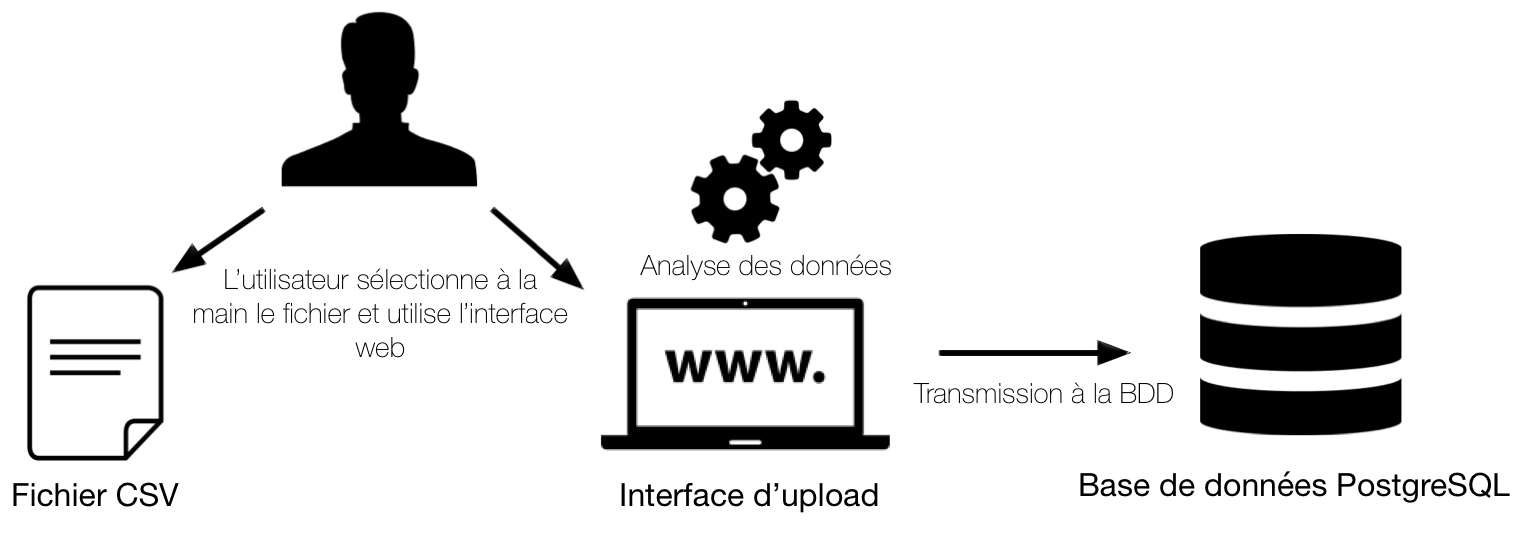
\includegraphics[scale=0.57]{images/datafit.png}
\captionof{figure}{Principe de l'interface d'upload}
\label{interface_upload}
\end{center}


Le diagramme de cas d'utilisation \ref{arena_pricing_use_case} page \pageref{arena_pricing_use_case} détail les différentes possibilités d'envoie de données pour un utilisateur :
\begin{itemize}
	\item[\textbullet] Via un fichier CSV d'export contenant les données billétteries, le client importe envoie ce fichier sur l'interface d'upload du site.
	\item[\textbullet] Via une API, il peut demander directement le "rapatriement" des données 
\end{itemize}


\begin{center}
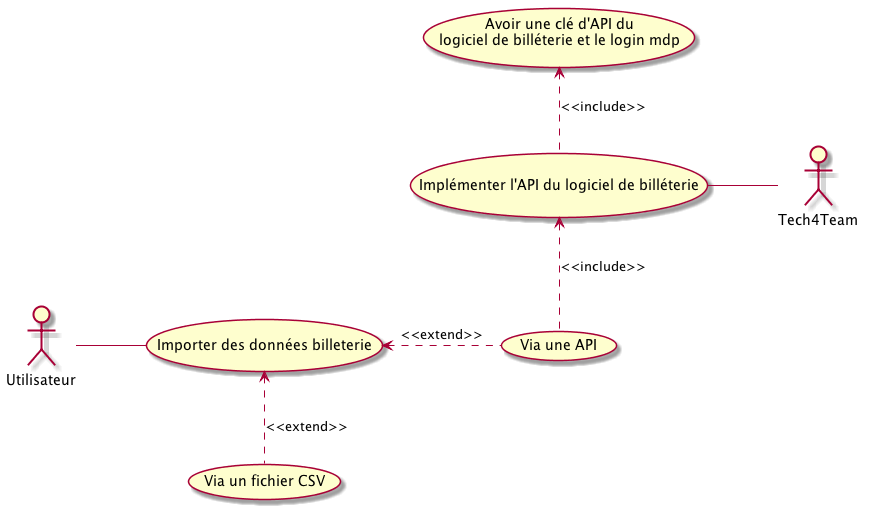
\includegraphics[scale=0.57]{images/arenapricing-use-case.png}
\captionof{figure}{Diagramme de cas d'utilisation de l'interface d'upload d'ArenaPricing}
\label{arena_pricing_use_case}
\end{center}


\subsection{Première réalisation du front d'importation}

Pour réaliser ce site web d'importation nous avons décidé après discussion avec le lead developper d'utiliser le langage Python. Ce langage permet de développer rapidement et dispose de nombreux modules s'ajoutant aux fonctions de base. Il est ainsi aisé de parser un fichier CSV. J'ai également utilisé le microframework Flask pour créer les pages web en elle même et servir de serveur web. Pour le design du site, j'ai utilisé le framework Zurb Foundation afin d'avoir une identité visuelle cohérente avec le reste du site ArenaMetrix. 

\begin{center}
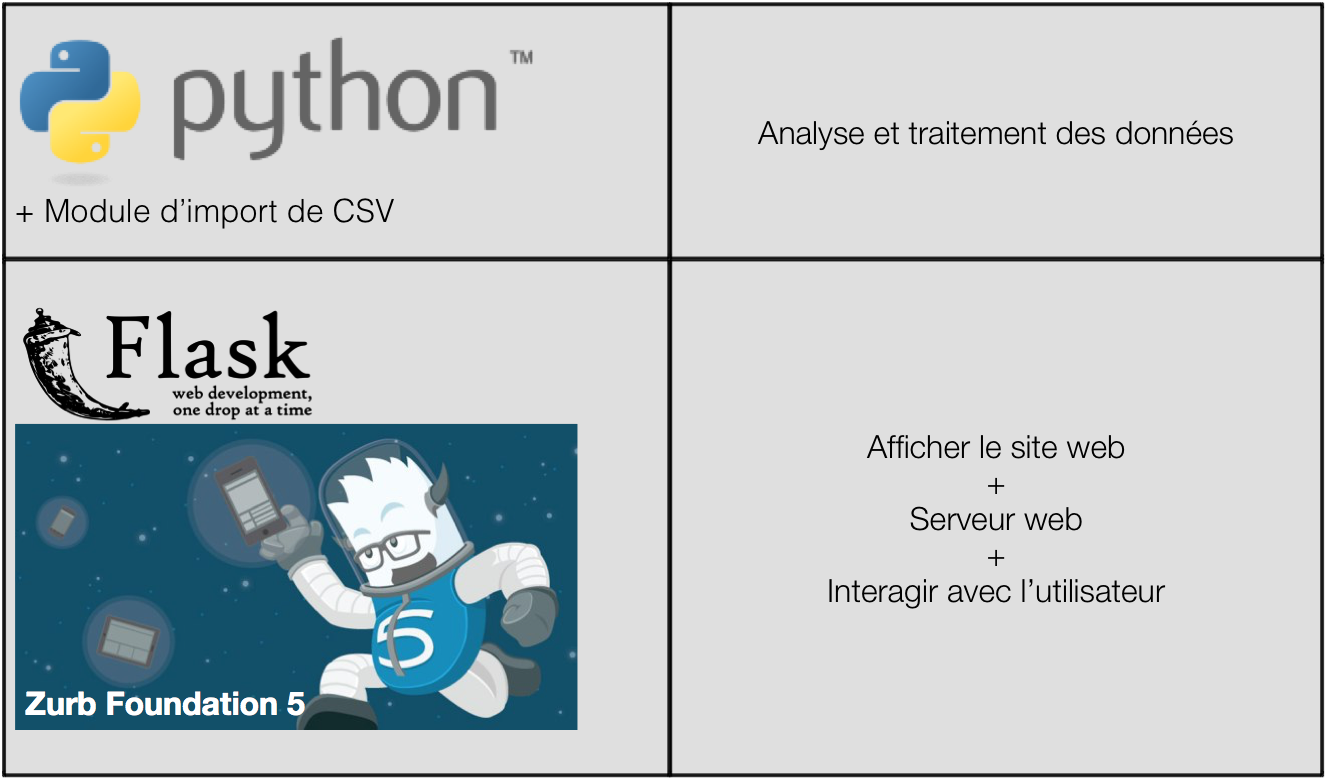
\includegraphics[scale=0.6]{images/datafit2.png}
\captionof{figure}{Téchnologies utilisées pour le front}
\label{interface_upload_tech}
\end{center}

\subsubsection{L'interface homme-machine obtenue}

Comme nous pouvons le voir sur l'impression d'écran \ref{front_upload} page \pageref{front_upload} l'interface permet à l'utilisateur d'envoyer un fichier CSV préalablement sélectionné.
En plus du nom de l'organisation, nous affichons le type d'événement correspondant au fichier envoyé ainsi que le logiciel de billetterie d'où provient l'export. \\

\begin{center}
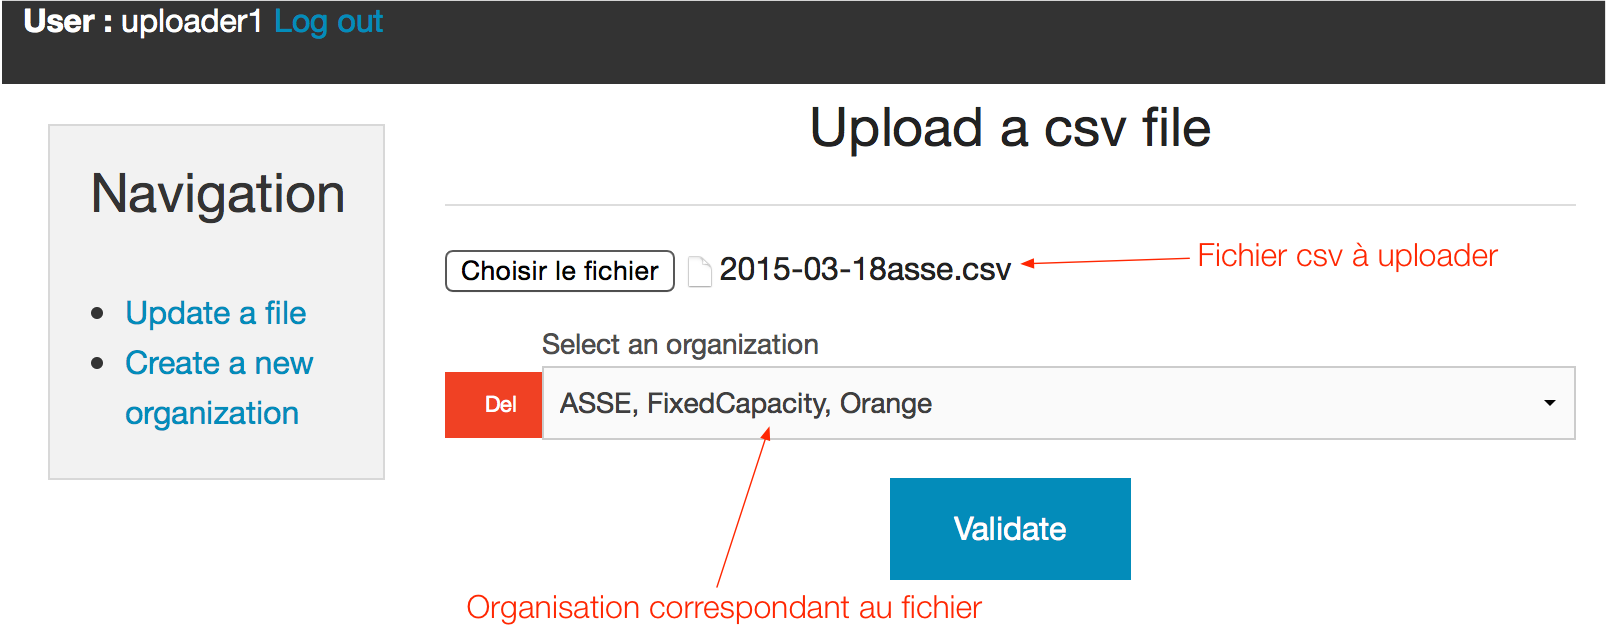
\includegraphics[scale=0.6]{images/front1.png}
\captionof{figure}{Front d'upload d'un fichier CSV}
\label{front_upload}
\end{center}

\subsubsection{Parsing des données en Python}
Pour parser les fichiers CSV j'utilise le module natif CSV. Le principal problème avec les fichier CSV est l'encodage, parfois c'est du UTF-8, d'autres fois du latin1 ou encore du windows-1252. Le module $chardet$ permet de détecter l'encodage d'un fichier.
\\


\lstset{style=custompython}
\begin{lstlisting}
f = open(p_path_file, 'rb')
charset_char = f.read(10000) #read 10000 first characters to detect charset
f.close()
charset = chardet.detect(charset_char)
with open(file_path, 'r', encoding=charset['encoding']) as f:

	#read csv file with csv module
	dict_csv = csv.DictReader(f, delimiter=';', quoting=csv.QUOTE_ALL)
	
	#use strategy design pattern with Secutix object
	secutix = ParsingStrategyContext(Secutix())	
	
	#parse dictionay and send organization name, event date, export date
	secutix.parse_file(dict_csv, o_name, e_date, export_date)

#ask object to send data to the ruby. e_type is event type 
reason = secutix.upload_data(e_type)
return reason
\end{lstlisting}
\captionof{lstlisting}{Code analysant le fichier CSV}

\leavevmode \\
La fonction open permet d'ouvrir le fichier $file\_path$, ensuite je récupère le dictionnaire associé à au fichier CSV avec $csv.DictReader$. La méthode $parse\_file$ permet de générer le dictionnaire avec les informations des tickets/achats comme le montre la figure \ref{dict_csv} page \pageref{dict_csv}, nous obtenons finalement une liste de dictionnaire ou chaque entrée de la liste est une ligne du fichier CSV. 

\begin{center}
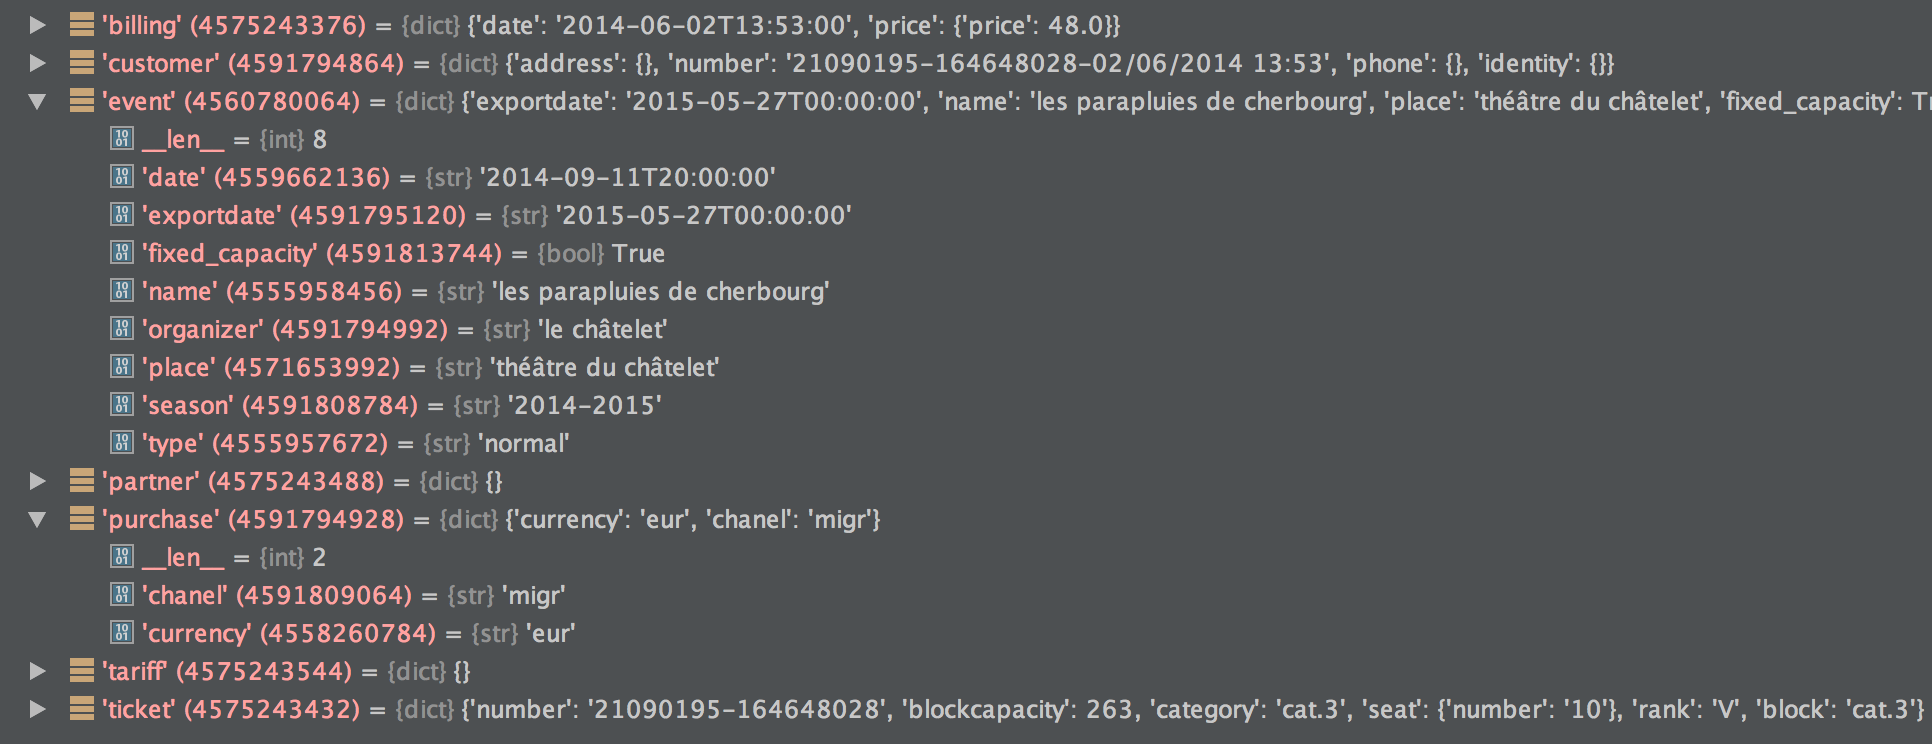
\includegraphics[scale=0.45]{Images/dict_tickets.png}
\captionof{figure}{Dictionnaire récupéré pour une ligne du fichier CSV}
\label{dict_csv}
\end{center}

D'un point de vue architecture de l'application j'utilise le design pattern strategy. Ce design pattern est utile lorsqu'un objet peut effectuer plusieurs traitements différents, dépendant d'une variable ou d'un état.

L'implémentation de ce design pattern peut être visualisé sur le diagramme figure \ref{stategy_pattern} page \pageref{dict_csv}.

\begin{center}
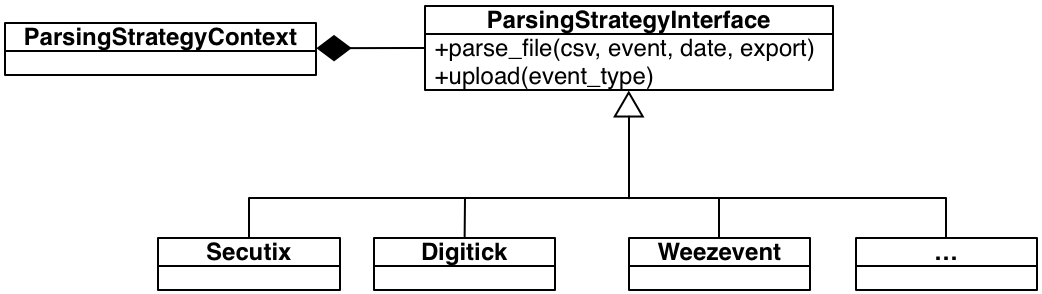
\includegraphics[scale=0.75]{Images/StrategyPattern.png}
\captionof{figure}{Design pattern strategy}
\label{stategy_pattern}
\end{center}


\subsubsection{Problèmatique posée par ce logiciel}
Après avoir testé le logiciel d'importation avec de nombreux clients, il s'avère que les fichiers fournis ne sont pas générique. \\
Les noms des colonnes ne sont pas les mêmes en fonction des exports alors que le logiciel de billetterie est identique et dans certains cas le changement apparait pour un même client d'une saison à l'autre. \\
On se rend donc rapidement compte que nous ne pouvons pas créer un script unique par logiciel de billetterie.
\\

La partie front en Flask n'est actuellement plus utilisée, mais le python qui permet de parser les données et utilisé pour les clients qui n'ont pas d'API et qui uploadent donc des fichiers CSV sur un serveur FTP. 


\subsection{Deuxième itération pour le logiciel d'import des fichiers}
Nous décidons de repenser notre logiciel pour que le client désirant envoyer un fichier CSV puisse spécifier sur l'interface les champs qu'il souhaite importer.

Comme le montre l'image \ref{draft_front_import2} page \pageref{draft_front_import2} du premier draft que j'ai réalisé, le client doit maintenant faire un travail d'association entre les champs présents dans le fichier CSV leur correspondance réelle. 

\begin{center}
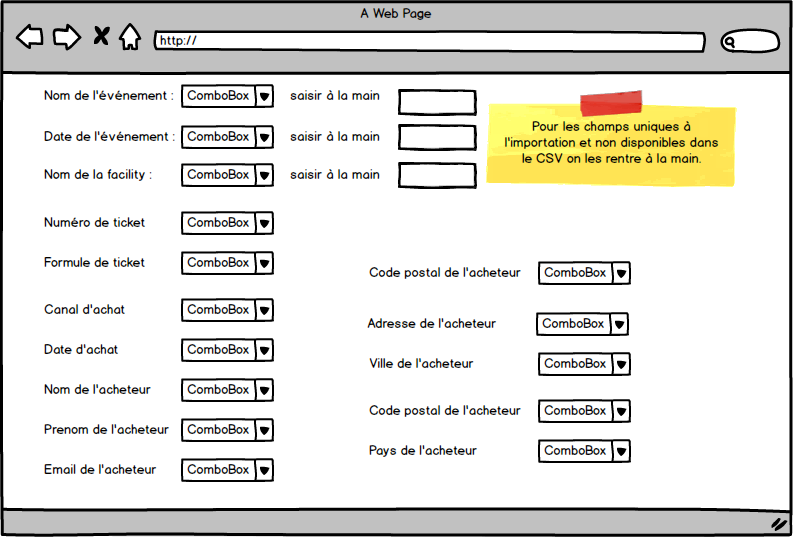
\includegraphics[scale=0.55]{images/front3.png}
\captionof{figure}{Premier draft du logiciel d'importation 2.0}
\label{draft_front_import2}
\end{center}


\subsubsection{Création de l'IHM}
Pour réaliser l'interface d'upload j'ai utilisé le framework Ruby On Rails afin de pouvoir intégrer facilement et directment la page d'upload au reste du site. Après réflexion, il est plus simple pour nous de maintenir le logiciel principal avec une seule et même technologie : le Ruby. Le Python n'est actuellement utilisé que pour les scripts.

\begin{center}
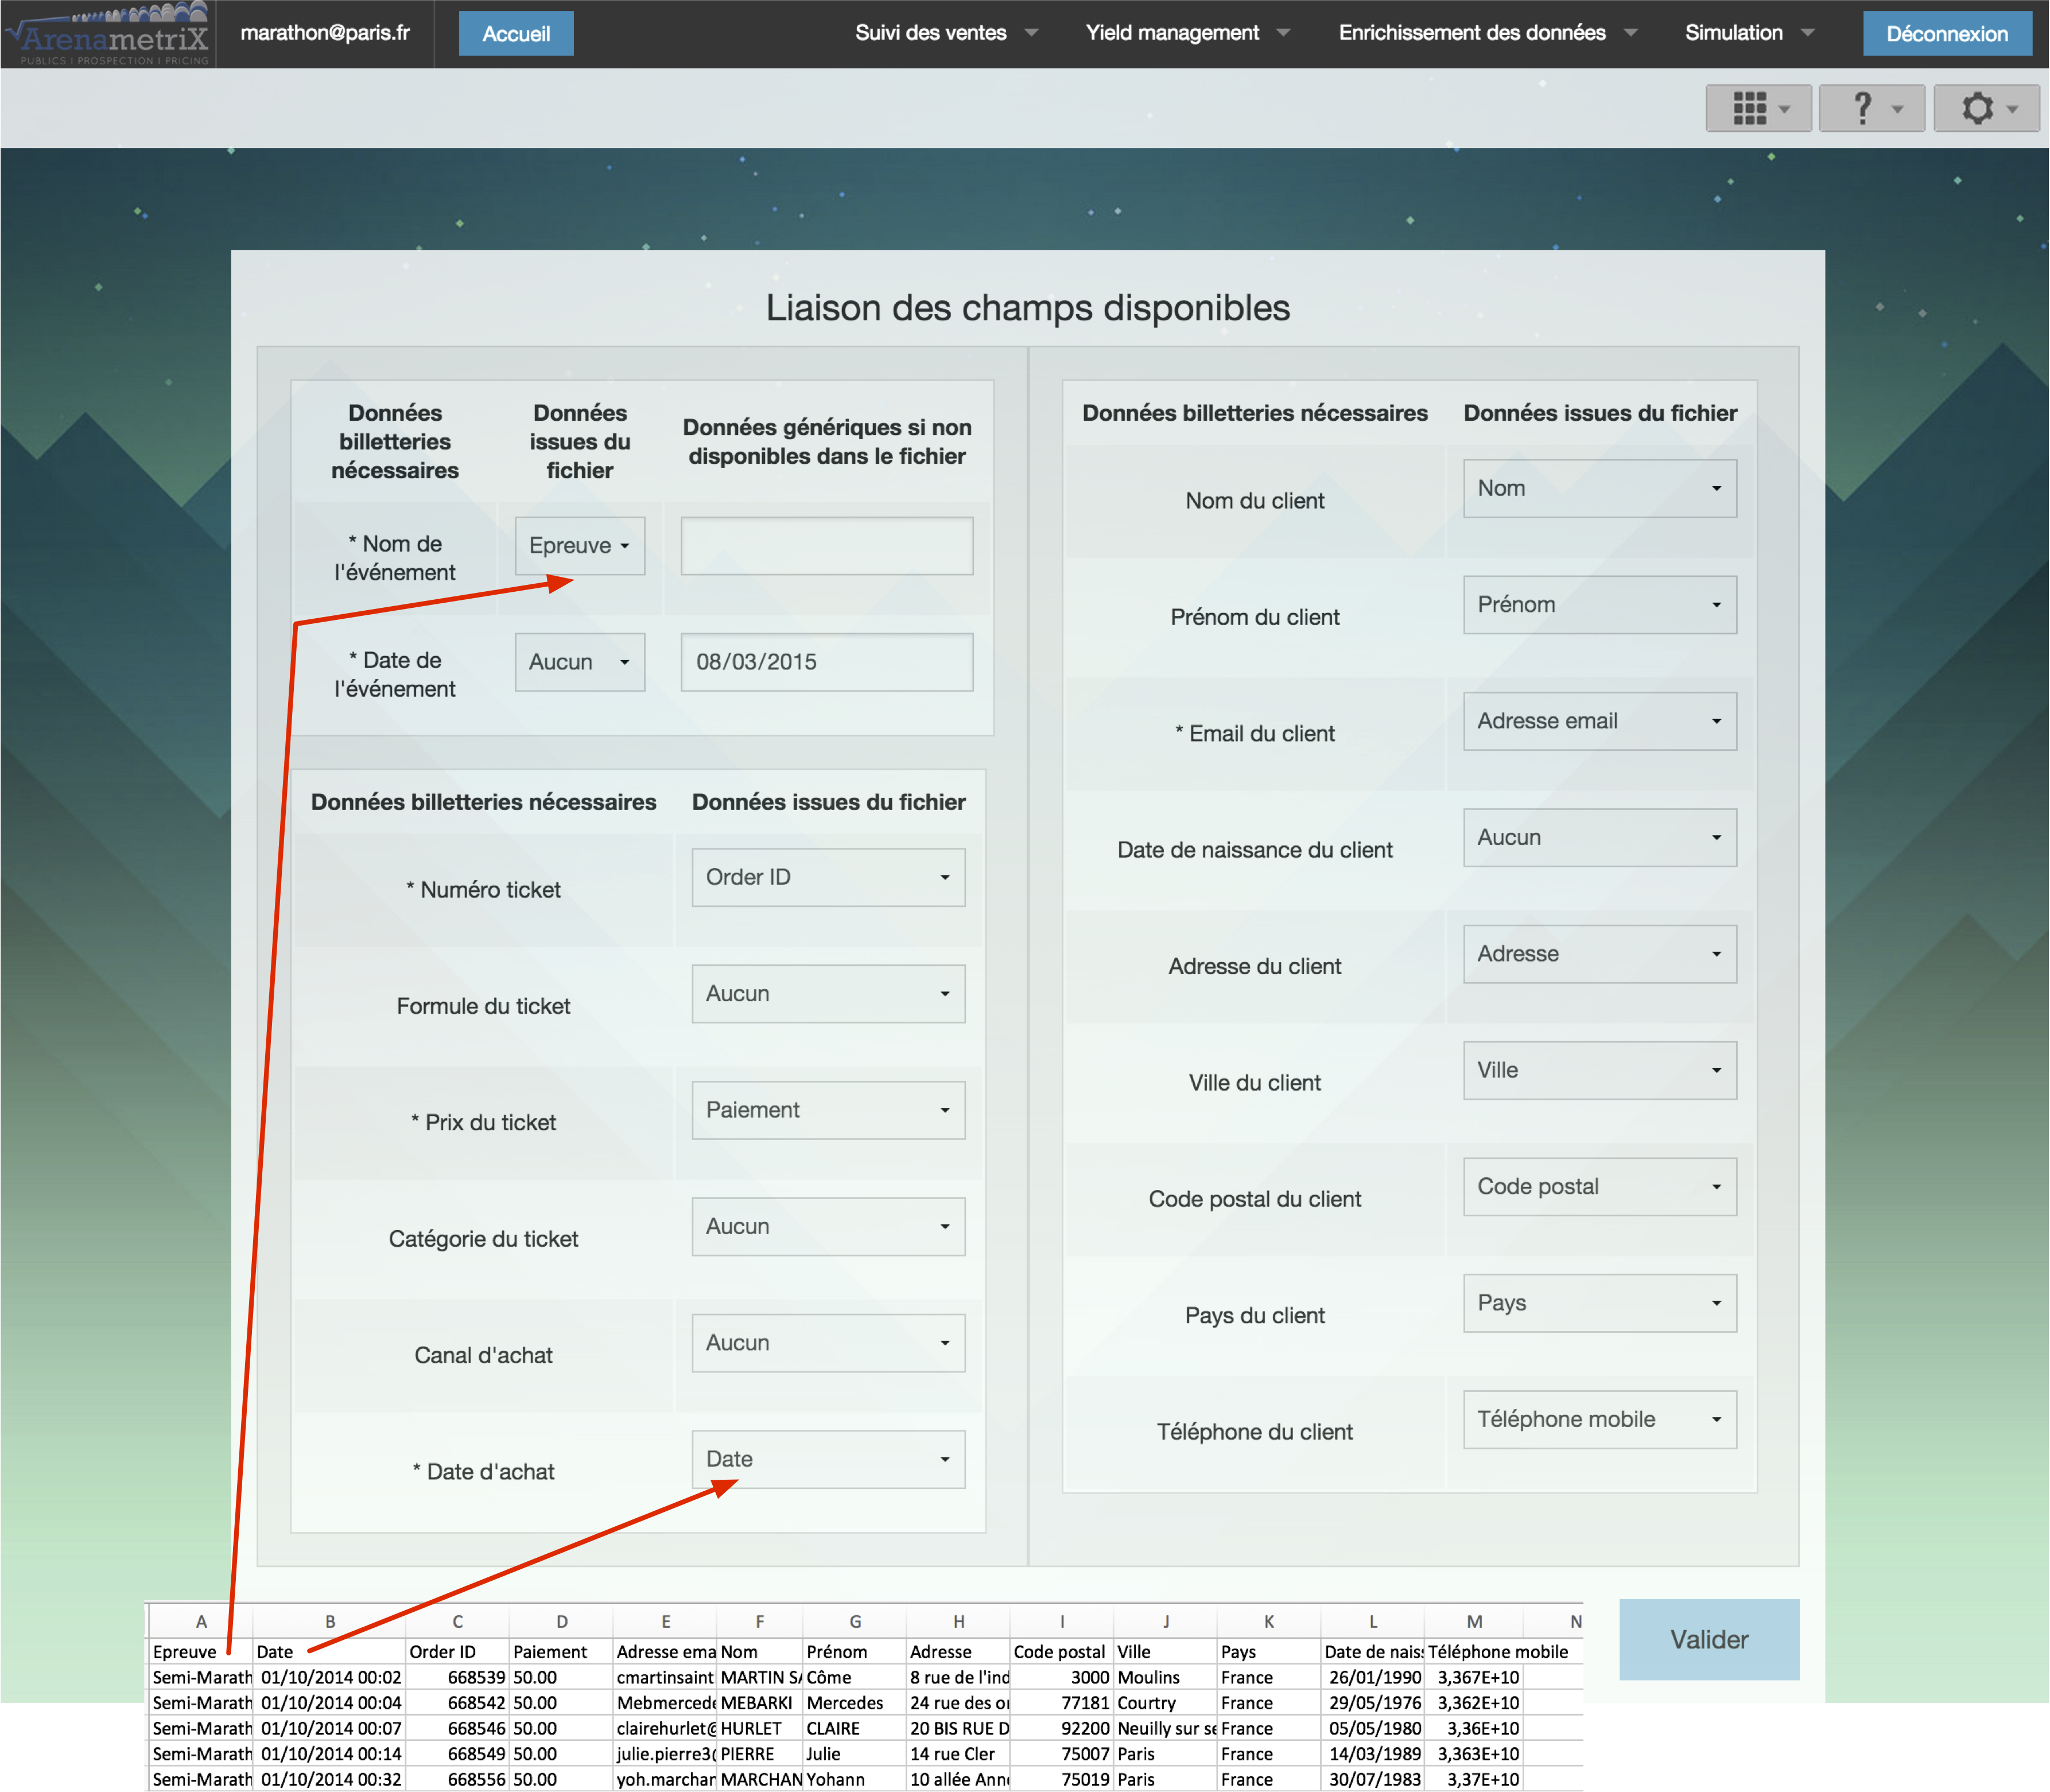
\includegraphics[scale=0.37]{images/final_front2.png}
\captionof{figure}{Logiciel d'importation des clients}
\label{final_front_import2}
\end{center}

J'obtiens finalement le front-end \ref{final_front_import2} page \pageref{final_front_import2}, comme nous pouvons le voir avec le fichier CSV de test les champs sont mappés ensemble. Si la donnée n'est pas présente, une insertion vide se fait en base de données. Les champs marqués avec une étoile sont indispensables. Certains champs si ils sont uniques à l'import, comme le nom de l'événement et la date peuvent être inscrits à la main s’ils ne sont pas fournis dans le fichier CSV.


\subsubsection{L'importation des fichiers CSV}

Afin d'importer les données dans le logiciel de billetterie j'utilise l'ORM ActiveRecord.

\lstset{style=customruby}
\begin{lstlisting}
begin
  country = Pricing::Country.find_by!(name: customer_country_to_ins)
rescue ActiveRecord::RecordNotFound 
  country = Pricing::Country.new(name: customer_country_to_ins)
end
country.save
begin
  department = Pricing::Department.find_by!(name: customer_zip_to_ins, country: country)
rescue ActiveRecord::RecordNotFound
  department = Pricing::Department.new(name: customer_zip_to_ins,  country: country)
end
department.save
begin
  city = Pricing::City.find_by!(name: customer_city_to_ins, department: department)
rescue ActiveRecord::RecordNotFound
  city = Pricing::City.new(name: customer_city_to_ins,  department: department)
end
city.save
\end{lstlisting}
\captionof{lstlisting}{Exemple de code insérant une adresse}
\leavevmode \

Avant d'insérer une donnée, je vérifie si elle est présente, si ce n'est pas le cas je rescue l'exception et j'insère la donnée. 
L'ORM ActiveRecord permet de s'astreindre des contraintes habituelles du SQL, lorsque je fais $coutry: country$ lors d'une intention de département l'ORM comprend qu'il doit lier $country$ comme clé étrangère de $département$.

\subsection{Les API des logiciels billetteries}
Différentes approches pour importer les données sont possibles : 
\begin{itemize}
  \item[\textbullet] Le client nous donne le login et mot de passe de son logiciel billetterie : nous faisons l'extraction d'un fichier CSV et nous l'importons à la main dans la base de données. 
  \item[\textbullet] Le client envoie son fichier CSV par mail : nous l'importons à la main dans la base de données (et lui redemandons le fichier si il manque des champs...).
  \item[\textbullet] Le client dépose son fichier CSV sur un serveur FTP : un script Python est chargé de régulièrement scanner ce serveur FTP et d'importer les données s'il a un changement.
  \item[\textbullet] La société logiciel billetterie nous donne une clé d'API, ainsi avec le mot de passe et login du client nous pouvons accéder aux données en nous connectant directement à la base de données. C'est l'idéal pour nous, cela nous permet d'automatiser les imports.
\end{itemize}

Actuellement nous avons accès aux API des billetteries WeezEvent, Njuko et Digitick. 
Pour récupérer les données des API j'utilise le module request qui permet de faire des requêtes get.
\\ \\
Ainsi la requête suivante me permet de récupérer les événements d'une organisation :

\lstset{style=custompython}
\begin{lstlisting}
json_events = requests.get("https://api.weezevent.com/events",
                            params={'api_key': API_KEY,
                                    'access_token': token,
                                    'include_closed': True}
                          )
events = json_events.json()['events']
for event in events :
	#Traitemet
\end{lstlisting}
\captionof{lstlisting}{Récupération des événements sur l'API de weezevent}
\leavevmode \

À la fin de mon stage, nous avions accès a trois API de logiciel de billetteries : 
\begin{itemize}
  \item[\textbullet] WeezEvent pour les événements :
  \begin{itemize}
	\item Mondial du tatouage : un salon annuel pour les tatoueurs du monde entier
	\item File7 : Une salle de concert en région parisienne. 
	\item Rhum Fest : Un événement et une exposition sur le thème de rhum
  \end{itemize}
  \item[\textbullet] Njuko pour les événements :
  \begin{itemize}
  	\item Marathon de Paris
  \end{itemize}
  \item[\textbullet] Digitick pour :
  \begin{itemize}
  	\item Le musée Grévin
  \end{itemize}

\end{itemize}

\subsection{La base de données en elle même}
L'architecture de la base de données ArenaPricing peut être visualisée sur la figure \ref{arenapublic-1} de l'annexe page \pageref{arenapublic-1}.
\\

Cette base de données de la première forme normale car tous ses attributs de la base de données ont des valeurs simples (non multiples, non composées).
\\

Elle est également en deuxième forme normale car aucun attribut non clé ne dépend d'une partie de la clé.
\\

Et de troisième forme normale car aucun attribut non clé ne dépend d'un ou plusieurs attributs ne participant pas à la clé.



%TODO Parler des formes normales

		
%!TEX root =/Users/ludovicl/Dropbox/Cours/UTBM/P15/RapportStage/main.tex
\section{ArenaPublic}
Le logiciel ArenaPublic a pour but d'être un CRM amélioré, l'utilisateur doit pouvoir au travers de ce logiciel visualiser les données des clients en base de données. 
\\

À la différence de ArenaPricing où nous nous concentrons sur les tickets vendus, ici c'est le client qui est au centre de la base de données, à terme cette application doit permettre à l'utilisateur d'afficher des données de scoring \footnote{Le scoring (statistique) est un ensemble de méthodes conduisant à un classement d'individus au sein de groupes préalablement définis ou de segmentation.}.
\\

La base de données ArenaPublic est reliée à la base de données ArenaPricing par l'intermédiaire de la base ArenaMetrix. ArenaMetrix est visible en annexe \ref{arenametrix-db} page \pageref{arenametrix-db}, cette base identifie l'utilisateur du site web et gère l'accès aux pages avec la gem TheRole.

\subsection{Première approche et problème technique}
Après avoir défini avec les statisticiens un modèle de base de données relationnelle que nous pensons générique, nous nous rendons compte qu'il nous faut plus de souplesse sur la structure. En effet, les données à scorer et à afficher peuvent varier d'un utilisateur à l'autre et évoluent en fonction de la demande de l'utilisateur et des statisticiens.

\begin{center}
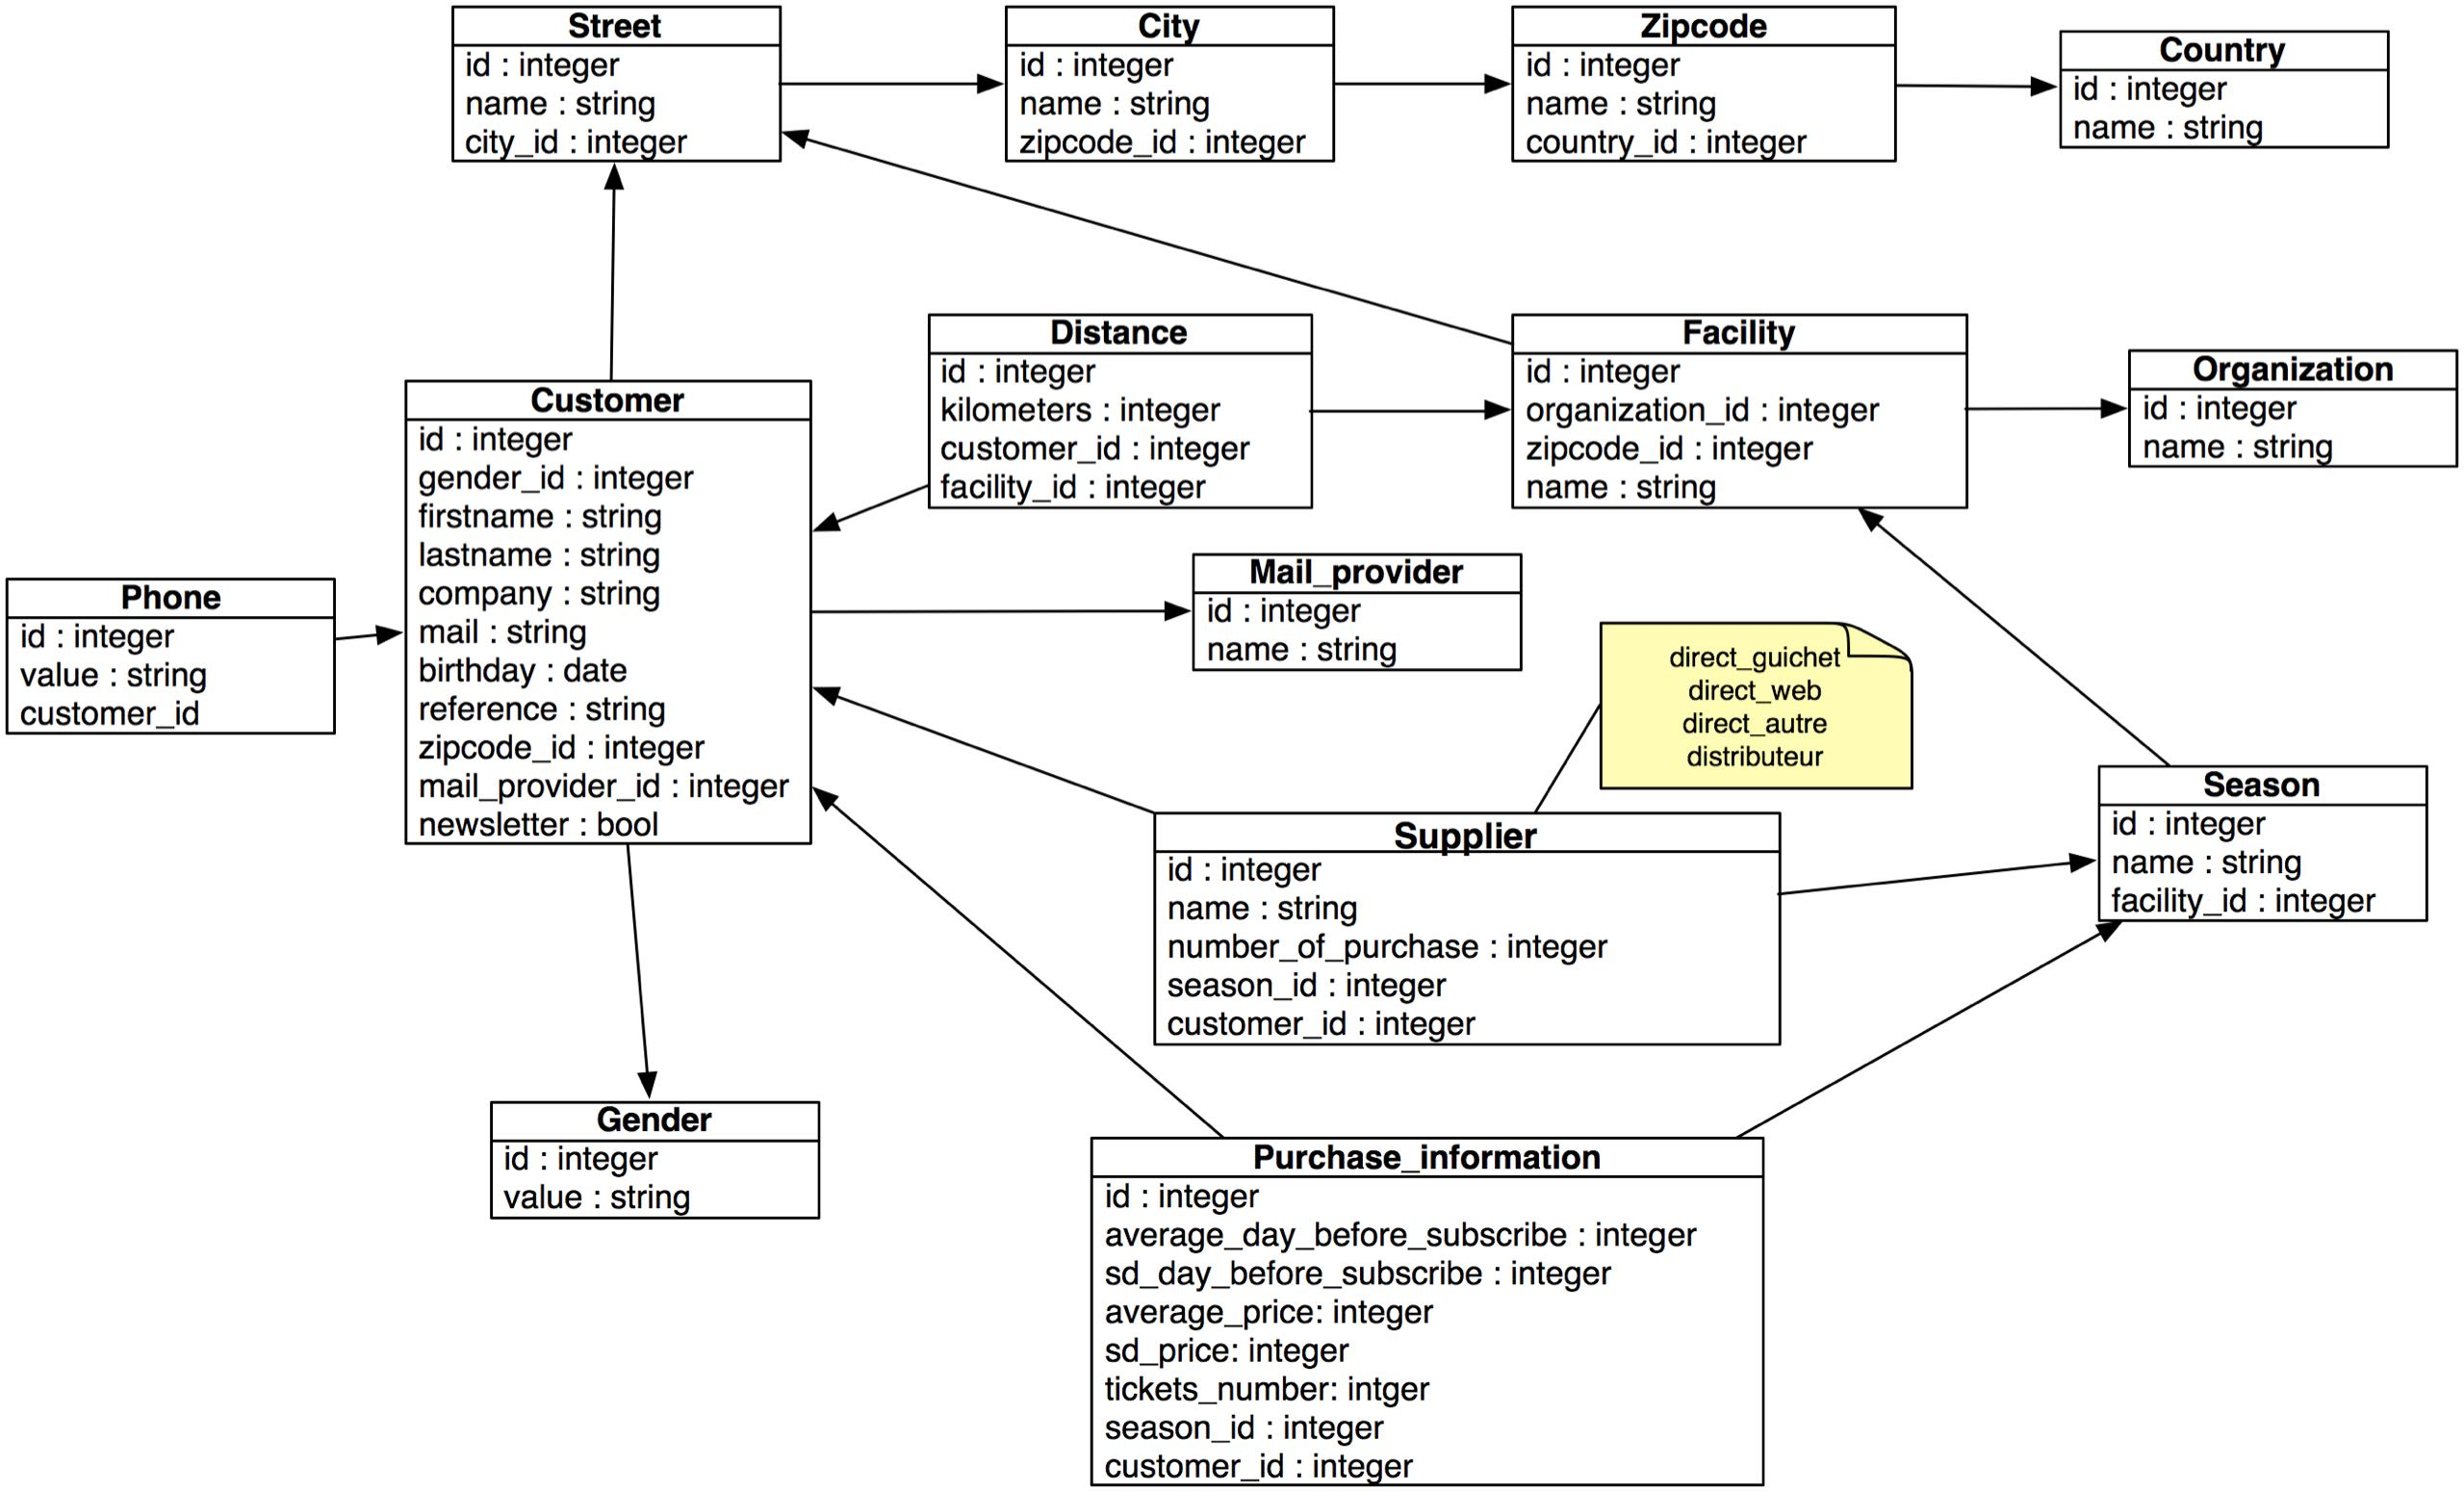
\includegraphics[scale=0.2]{images/arenapublic-1.jpg}
\captionof{figure}{Premiere architecture de la base de données ArenPublic}
\label{arenapublic-1}
\end{center}


Comme le montre l'architecture de base de données \ref{arenapublic-1} page \pageref{arenapublic-1} des données comme des écarts types et des moyennes dans les tables "Supplier" et "Purchase information" sont calculées à la volé et utilisés par les statisticiens. Le problème est qu'il nous faut pouvoir ajouter de nouvelles données facilement en fonction de la demande du client ou du besoin des statisticiens.
\\

Nous décidons donc d'utiliser en complément de la base de donnée SQL une base de base de données de type NoSQL \footnote{Not only SQL} qui permet de rajouter des informations "à la volée" sans modifier la structure de la base de données. 

\subsection{Implémentation technique}
Pour la base de données NoSQL nous voulions uns solution simple à mettre d’oeuvre de type clé valeur. Nous utilisons donc le système de base de données décentralisée Riak qui permet de stocker des informations de type clé valeur dans un bucket.

\begin{center}
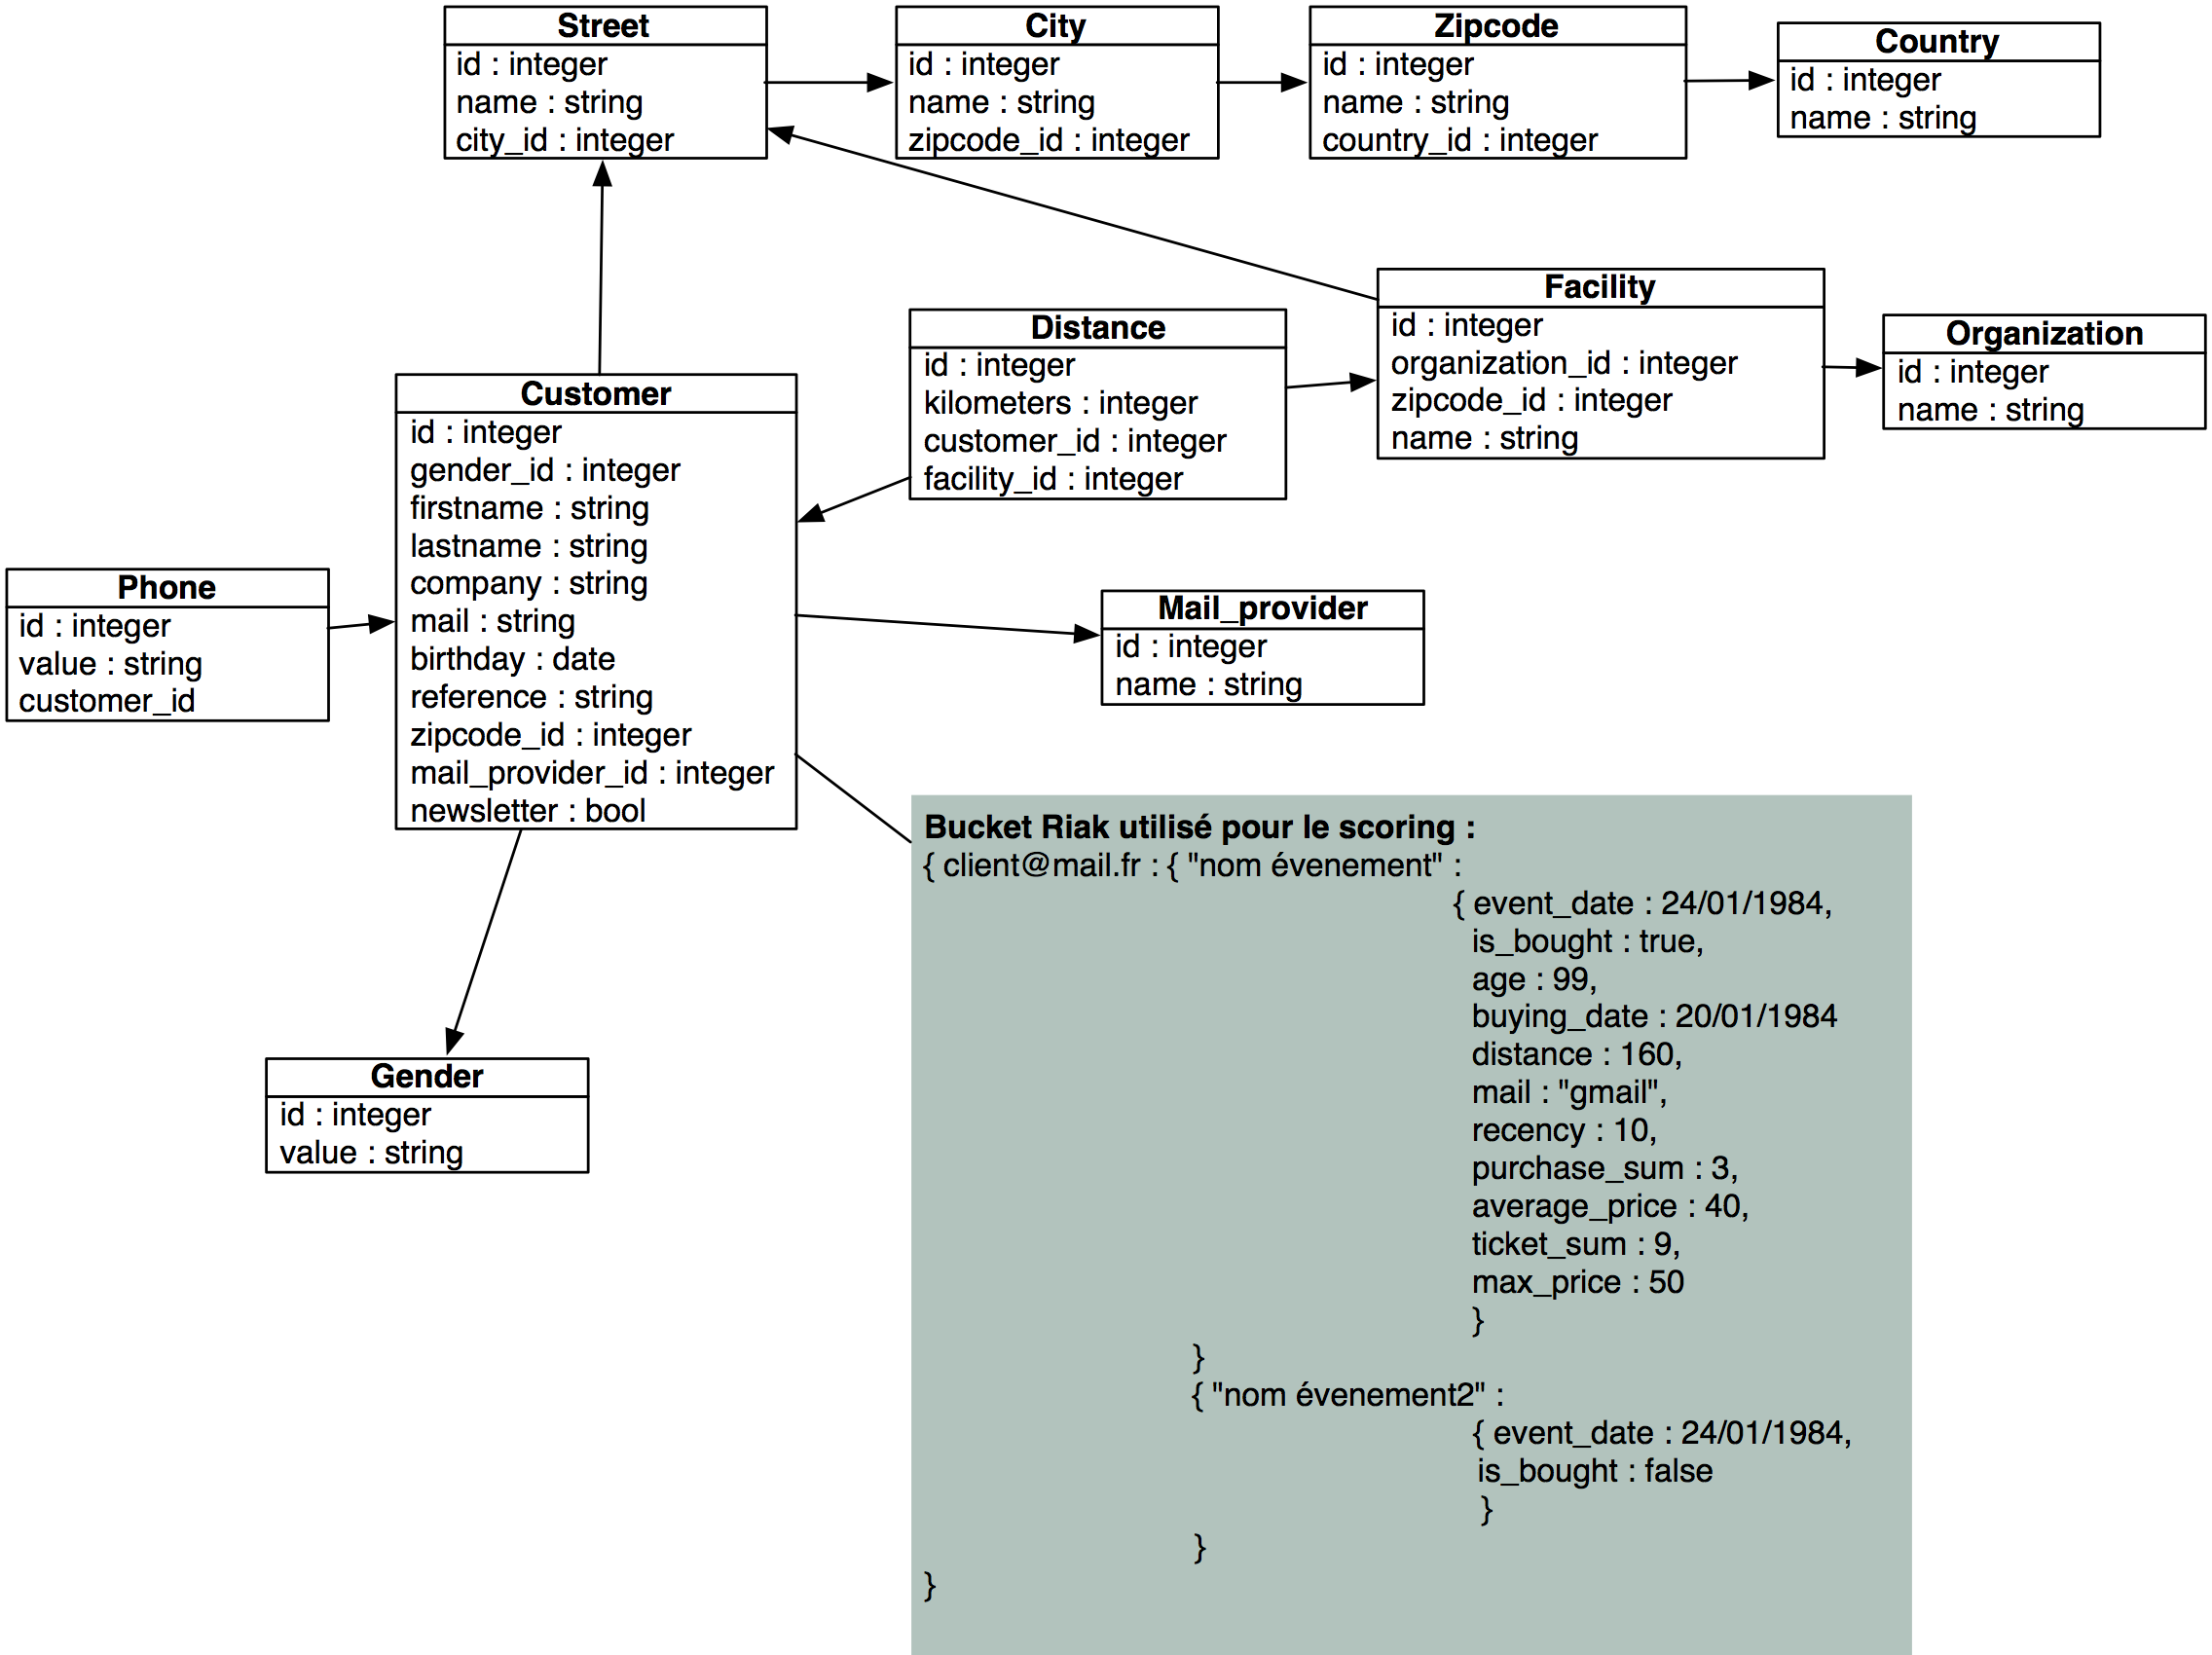
\includegraphics[scale=0.62]{images/arenapublic-2.png}
\captionof{figure}{Architecture finale de la base de données ArenaPricing}
\label{arenapublic-2}
\end{center}

Finalement nous obtenons l'architecture de base de données visible en \ref{arenapublic-2} page \pageref{arenapublic-2}.

La clé du Riak est l'adresse mail du client dans la base de données, il s'agit de la seule valeur vraiment indispensable pour identifier les clients de manière unique.

\subsection{Remplissage de la base de données}

Pour remplir la base de données ArenaPublic nous pouvons utiliser deux méthodes : 
\begin{itemize}
  \item[\textbullet] Un front d'upload qui permet d'envoyer un fichier CSV avec les clients abonnés pour une saison spécifique.
  \item[\textbullet] En allant piocher directement dans la base de données ArenaPricing.
  \end{itemize} \
  
\begin{center}
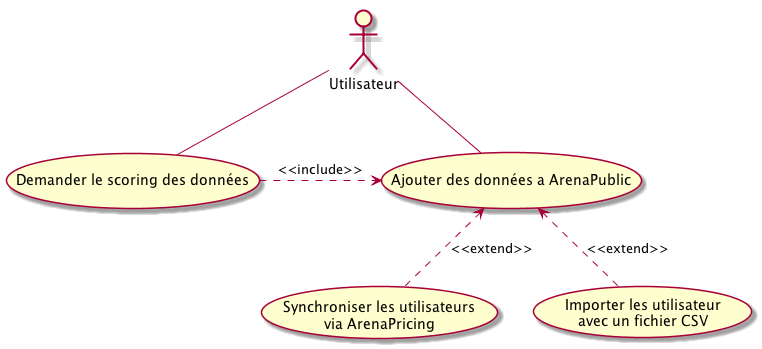
\includegraphics[scale=0.6]{images/arenapublic-use-case.png}
\captionof{figure}{Diagramme des cas d'utilisation de ArenaPublic}
\label{arenapublic_use_case}
\end{center}

Le diagramme des cas d'utilisation \ref{arenapublic_use_case} page \pageref{arenapublic_use_case} montre les différentes possibilités pour l'utilisateur d'importer des données relatives aux consommateurs afin de les scorer.
\begin{itemize}
	\item[\textbullet] Synchronisation des données depuis ArenaPricing 
	\item[\textbullet] Importation des données depuis un fichier CSV 
\end{itemize}
\leavevmode \\

Pour ma part j'ai essentiellement travaillé sur la synchronisation et l'agrégation des données depuis ArenaPricing. 
\\

Pour faire cela j'ai utilisé le langage Python, car il permet de facilement gérer des dictionnaires et de nombreux modules mathématiques sont disponibles pour pour fournir au statisticien des données aussi complètes que possible. Il ne leur reste ainsi qu'à les analyser.

\begin{center}
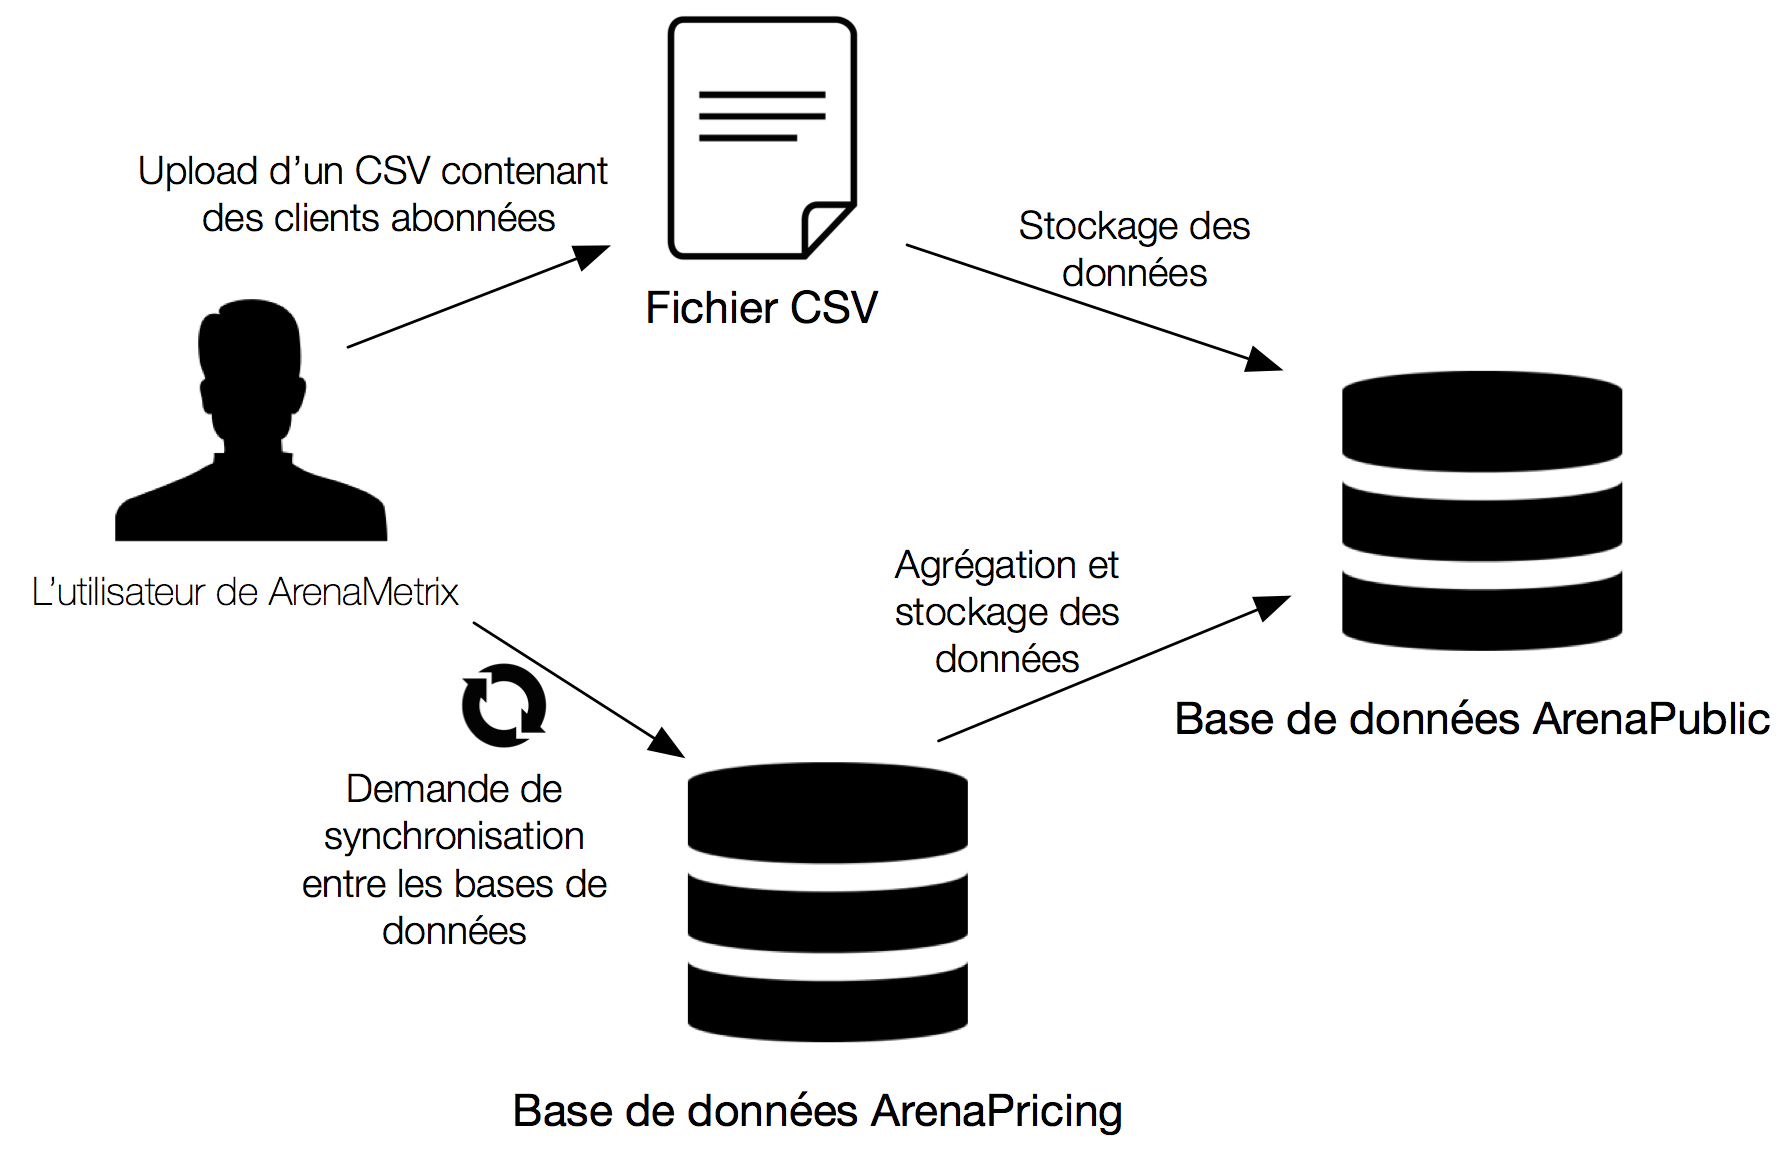
\includegraphics[scale=0.7]{images/public-to-pricing.png}
\captionof{figure}{Remplissage de la base de données ArenaPicing}
\label{public-to-pricing}
\end{center}

Comme le montre la figure \ref{public-to-pricing} page \pageref{public-to-pricing} il est possible pour l'utilisateur d'envoyer ses données au choix depuis un fichier CSV ou en synchronisant les données avec la base de données ArenaPricing. 
\\

La synchronisation des données avec ArenaPricing permet la réalisation d'un CRM à partir de données billéterie, d'un point de vue commercial ArenaPublic est uniquement disponibles pour le client ayant souscrit aux deux offres. 
\\

Tech4Team propose ainsi deux offres de scoring différentes : 

\begin{itemize}
  \item[\textbullet] Scoring sur le réabonnement : pour les clients nous fournissant des données abonnées. 
  \item[\textbullet] Scoring sur l'achat : pour les clients ayant des données dans ArenaPricing  
\end{itemize} 



\subsection{Enrichissement des données}
Lors de l'agrégation des données de ArenaPricing dans ArenaPublic en plus de faire les calculs servant aux statisticiens, j'ai enrichi les données disponibles afin d'offrir plus de possibilités au statisticien.
\subsubsection{Détermination du sexe}
Ajout du sexe de la personne en fonction du prénom lorsque l'information n'est pas disponible :
our réaliser cet enrichissement de données, j'ai utilisé le module 
\href{https://github.com/ferhatelmas/sexmachine/}{SexMachine}
Ce module retourne male, female, mostly\_male, mostly\_female ou andy en fonction du prénom passe en paramètre.

\lstset{style=custompython}
\begin{lstlisting}
>> import sexmachine.detector as gender
>>> d = gender.Detector()
>>> d.get_gender(u"Bob")
u'male'
>>> d.get_gender(u"Sally")
u'female'
>>> d.get_gender(u"Pauley") # should be androgynous
u'andy'
\end{lstlisting}
\captionof{lstlisting}{Exemple d'utilisation de SexMachine}
\leavevmode \\
Le problème avec le module officiel de SexMachine répertorié sur pypi est qu'il est compatible uniquement avec la version 2.7 de Python. Hors nous utilisons Python 3.X pour l'ensemble de nos logiciels et scripts Python. 

J'ai donc modifié SexMachine pour le rendre compatible avec Python 3.X. Le code source de la version modifié est disponible sur mon repository Github : \href{https://github.com/ludovicl/sexmachine}{https://github.com/ludovicl/sexmachine}.

\subsubsection{Calcul de la distance}

Pour enrichir les données des clients nous calculons la distance entre l'adresse de l'acheteur et l'adresse de l'infrastructure où a lieu l'événement.
Pour faire cela, j'utilise le module geocoder qui permet de wrapper différents sites de géocoding.
\\ \\
Après plusieurs tests j'utilise l'API de tomtom, car elle me donne les meilleurs résultats pour la France et n'a pas de limite d'utilisation.

\lstset{style=custompython}
\begin{lstlisting}
>>> import geocoder
>>> location_customer = geocoder.tomtom('Paris')
>>> location_facility = geocoder.tomtom('12 Rue Thierry Mieg, Belfort')
>>> geocoder.distance(location_customer, location_facility)
359.0865720640995
\end{lstlisting}
\captionof{lstlisting}{Exemple d'utilisation de geocoder}
\leavevmode \\

\subsection{Implémentation de bout en bout}
Pour faire communiquer nos applications de bout en bout nous utilisons MessagePack : il s'agit d'un format de sérialisation binaire qui permet d'échanger des données comme en JSON.

Ainsi, comme le montre le diagramme \ref{scoring} page \pageref{scoring} pour le scoring : 

\begin{itemize}
  \item[\textbullet] Le client demande la synchronisation de sa base de données ticket ArenaPricing en cliquant sur un bouton
  \item[\textbullet] L'interface (Ruby on Rails) lance une requête put une URL d'écoute qui est lancée en Flask depuis DataProc
  \item[\textbullet] DataProc récupère les données d'ArenaPricing, les agréges et les enrichie
  \item[\textbullet] DataProc enregistre les nouvelles données dans les bases de données PostegreSQL et Riak d'ArenaPublic
  \item[\textbullet] Le client est notifié que les données sont maintenant dans ArenaPublic
  \item[\textbullet] Le client sélectionne les données qu'il veut scorer
  \item[\textbullet] Les données sont récupérées dans la base de données
  \item[\textbullet] Les données sont envoyées au logiciel de scoring écris en Python. Le logiciel de scoring écoute sur une URL grâce à une instance lancée en Flask
  \item[\textbullet] Le logiciel de scoring retourne les données à la WebInterface
  \item[\textbullet] La WebInterface unpack le MesagePack et affiche les données associées sous forme de graphiques. 
 

\end{itemize} 

\begin{center}
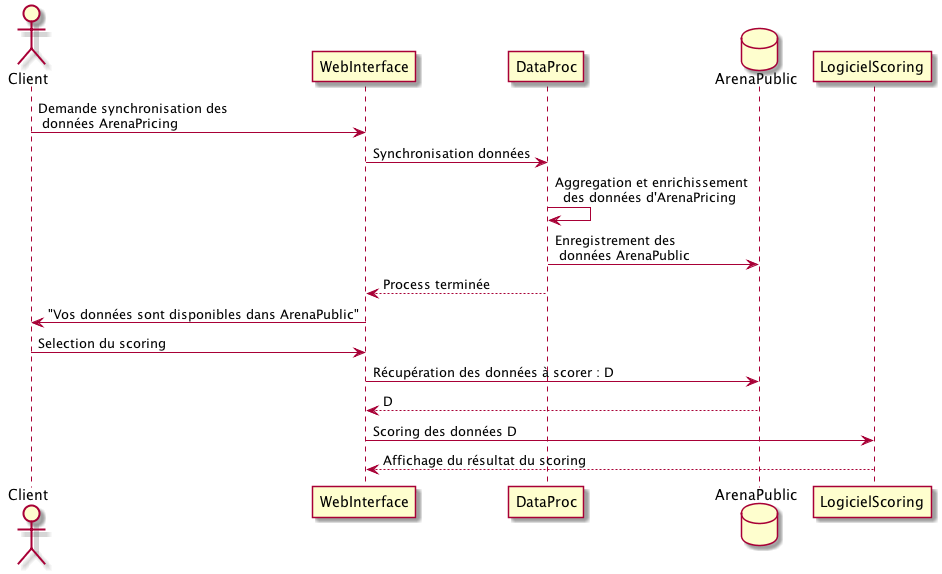
\includegraphics[scale=0.52]{images/scoring.png}
\captionof{figure}{Diagramme de séquence du scoring }
\label{scoring}
\end{center}


\section{Accueil et encadrement de stagiaires}
Début juin de nombreux stagiaires ont été recrutés, ces stagiaires étant en première années de l'ETNA je les ai donc managés et encadrée d'un point de vue technique :
\begin{itemize}
	\item[\textbullet] J'ai notamment eu sous ma responsabilité directe un stagiaire back-end qui a travaillé sur du Python et qui a fait la partie récupération des données exogènes comme la météo et le scrapping de certains sites. 
	\item[\textbullet] Un autre stagiaire était chargé de faire le front-end de ArenaPublic, j'ai donc direcemnt travaillé avec lui car je m'occupai de la partie Python et back-end Ruby de ce projet. Je l'ai également aidé pour les requêtes SQL à effectuer.
\end{itemize}

  



%!TEX root =/Users/ludovicl/Dropbox/Cours/UTBM/P15/RapportStage/main.tex
\chapter{Résultats et conclusion}

\section{Résultats}
Au terme de mon stage nous avons 15 clients en bêta test, la plupart des données sont encore importées à la main avec des fichiers CSV mais plus l'entreprise grandie et gagne en notoriété et plus nous avons accès aux API des logiciels de billetteries.
\\

D'ici quelques mois nous pourrons faire du temps réel sur la synchronisation des données et appliquer les modèles de prévisions à la volée.

\section{Conclusion}
Ce stage m'a permis de me familiariser davantage avec le monde de l'entreprise et cela de plusieurs manières :
	\begin{itemize} 
		\item[\textbullet] J'ai pu mettre en œuvre les connaissances acquises dans le domaine des bases de données dans un cadre professionnel
		\item[\textbullet]Je me suis initié au management en devant m'occuper de stagiaires
		\item[\textbullet]J'ai découvert le développement d'applications de type SaaS et les contraintes techniques que cela implique notamment au niveau des serveurs. 
	\end{itemize} 
\leavevmode \\
Après un premier stage effectué dans une entreprise de taille intermédiaire, je peux maintenant comparer ces deux mondes professionnels.
\\ \\
\textbf{Les entreprises de tailles intermédiaires}
\\
L'avantage que je trouve à travailler en tant que stagiaire dans ce genre d'entreprise est l'encadrement.
Les ingénieurs de ce type d'entreprise ont plus de disponibilités et peuvent nous guider dans l'exécution de certaines tâches. On peut s'appuyer sur leurs conseils. 

On sait exactement où l'on va, le travaille que l'on a faire est les collègues peuvent prendre du temps pour nous aider. Par contre on est juste y engrenage dans une machine beaucoup plus complexe.
\\ \\
\textbf{Les start-ups}
\\
L'encadrement est beaucoup moins présent, le travail à faire évolue au cours des semaines et des besoins des clients. Le nombre d'employés étant moindre le stagiaire a plus de responsabilités, il faut prendre des décisions, implémenter des fonctionnalités rapidement, on se forme on apprend sur le tas, c'est très formateur \\
Le seul risque est de prendre des mauvaises habitudes, mais avec tous les logiciels d'analyse de codes et les ressources à notre disposition on s'en sort.
\\
\\
\\

Mon stage s'est terminé le 31 juillet, l'entreprise m'a proposé un CDI que j'ai accepté. Mon rôle dans l'entreprise est de m'occupé de de la partie back-end et de la conception des bases de données.   

 

\appendix 
\setcounter{figure}{0}

\chapter*{Annexes}
\pagebreak[4]
  \global\pdfpageattr\expandafter{\the\pdfpageattr/Rotate 90}
\begin{landscape} 
\section*{Base de données ArenaPricing} \label{App:AppendixA}

\begin{center}
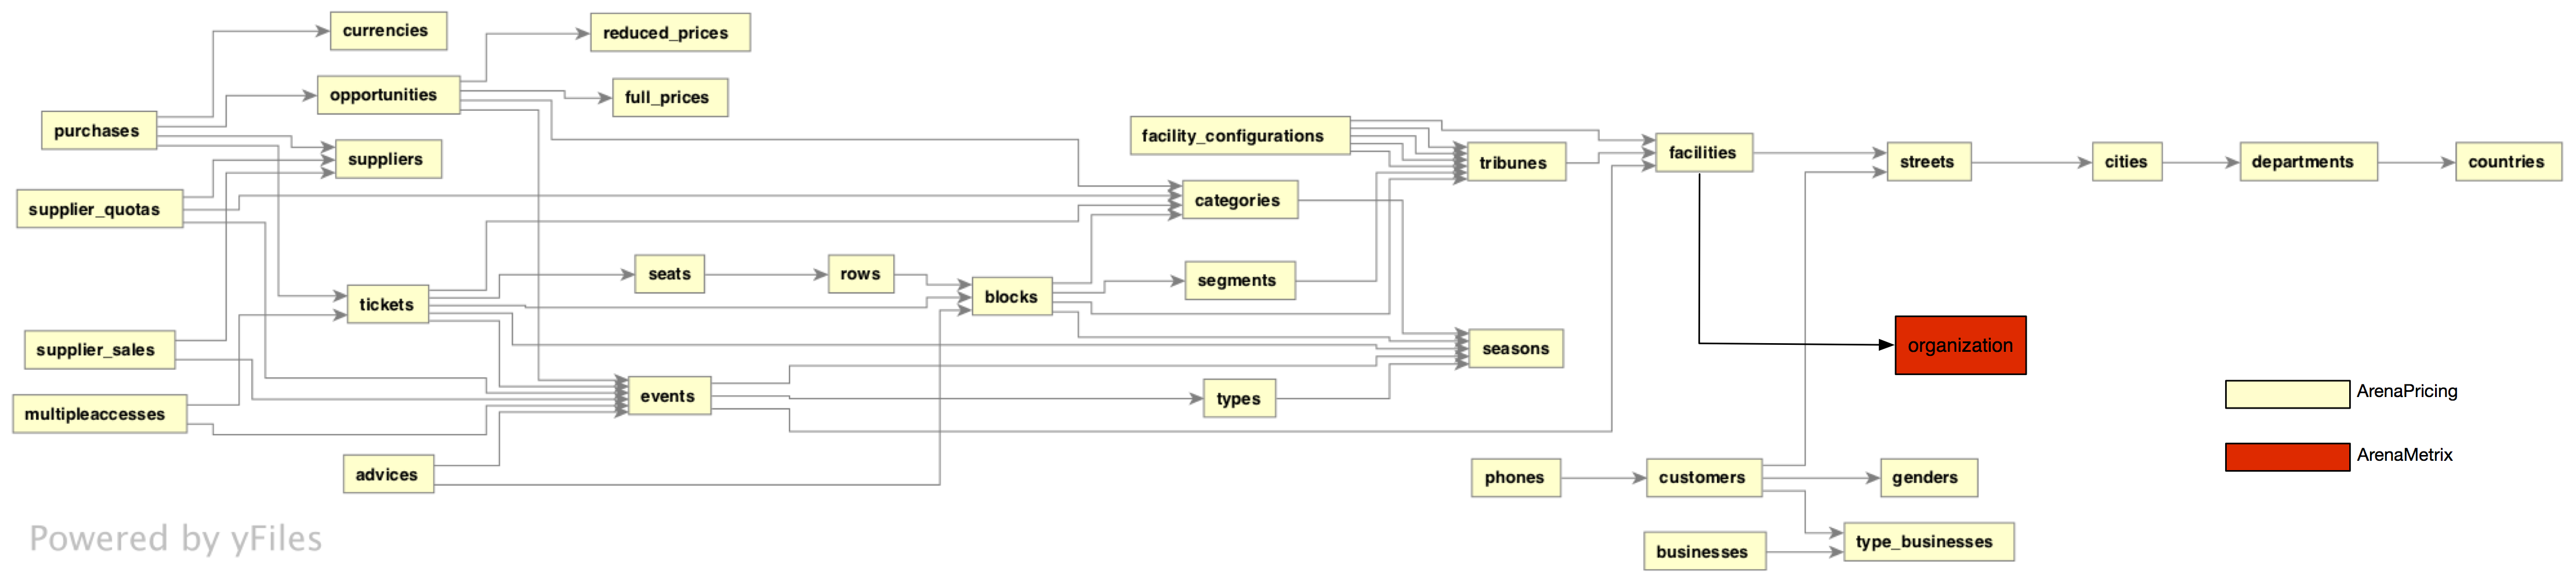
\includegraphics[scale=0.45]{images/ArenaPricing.png}
\captionof{figure}{La base de données ArenaPricing}
\label{arenapublic-1}
\end{center}

\end{landscape}

\pagebreak[4]
  \global\pdfpageattr\expandafter{\the\pdfpageattr/Rotate 0}

\mbox{}
\nocite{*}
\bibliographystyle{plain}
\bibliography{biblio}



\end{document}